%%
\bigheading{Tickets}
\authors{Gyula Horváth}{Gyula Horváth}{Gyula Horváth}
%%
\heading{Solution 1: request to seat selection}
Let $C(x)$ is the set of candidate requests for seat $x$:
$$C(x)=\{ r: r.first \leq x \leq r.last \textrm{ and r is not satisfied yet} \} $$
\noindent\textbf{Greedy choice:}\\
Choose the request with least last value.
\lstlang{cpp}\begin{lstlisting}
for (x=1;x<=N;){
    insert r into C where r.first=x;
    if (!C.empty(){
        r=C.top; C.pop();
        A[x]=r;
    }
    while (C.top().last==x) C.pop();
}
\end{lstlisting}
The running time of this algorithm is $O(M \, \log M)$ using priority queue for the implementation of the greedy choice, where $M$ is the number of the requests.

\heading{Solution 2: seat to request selection}
\noindent\textbf{Greedy choice:}\\
Take the requests in decreasing order of their first value and if there is a free seat in between the request's first and last value, choose the largest. Let $R[x]$ be the set of requests whose first seat is $x$. The operation $FindEmpty(a,b)$ returns the largest empty seat $d$, and if $a \leq d$ then mark $d$ as not free.
\lstlang{cpp}\begin{lstlisting}
   int sol=0;
   for(int x=n;x>0;x--){
      for(Req y:R[x]){
         int d=FindEmpty(x, y.last);
         if(x<=d){
            sol++;
            A[d]=y.id;
         }
      }
   }
\end{lstlisting}
\textbf{Proof of correctness.}\\
A problem instance is a par of sets $(S, R)$, where $S$ is the set of available seats and $R$ is the set of requests. A solution of a problem instance  $(S, R)$ is a partial function $A: S \rightarrow R$, the seat assignment. Assume that $A$ is an optimal solution. We show that the optimal solution can be modified such that it begins with the greedy choice. Let $r0$ be the greedy choice, i.e., $r0.first$ is largest among the requests. For the greedy solution $Ag$ $Ag[r0.last]=r0$ holds. If $A[r0.last]$ is not assigned, then set $A[r0.last]=r0$ and if for some $s$ $A[s]=r0$ delete this assignment. Assume that $A[r0.last]=r$ and $r \neq r0$. Therefore $r.first \leq r0.first$ and $r0.last \leq r.last$. If there is no seat $s$ such that $A[s]=r0$ then set $A[r0.last]=r0$. Otherwise change assignment by setting $A[s]=r$ and $A[r0.last]=r0$. The modified optimal solution includes the greedy choice. Denote the modified assignment by  $\overline{A}$.\\
Consider the reduced problem instance $(\overline{S}, \overline{R})$ where $\overline{S}=S-\{r0.last\}$ and $\overline{R}=R-\{r0\}$. The reduced assignment $A: \overline{S} \rightarrow \overline{R}$ is an optimal solution of the reduces problem instance, therefore $\overline{A}$ is an optimal solution of $(S,R)$
\heading{Implementation of the FindEmpty operation by Union-Find}
\begin{center}
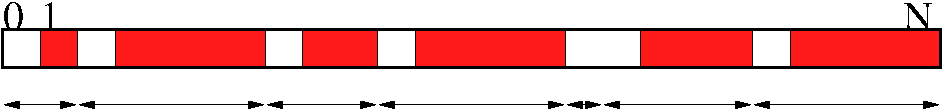
\includegraphics[height=1.5cm]{img/abra51.pdf}
\end{center}
Consider the disjoint intervals of the set of seats, such that the least element is a free seat and this is the only free seat in the interval.

The sets of request $R[x]$ can be represented by list, therefore the creation of the sets $R[x]$ requires $\Theta(M)$ time.\\
The running time of this algorithm is $O(M \, \alpha(N,M))$.
